% 2017-01-27 - Bruno Iran Ferreira Maciel - bifm@cin.ufpe.br
\documentclass[xcolor=table,smaller,aspectratio=169]{beamer}

% ----------------------------------------------------------
% Customização p/ o estilo bifm
% ----------------------------------------------------------
\usepackage{bifm}

% ----------------------------------------------------------
% Configura parâmetros p/ o estilo bifm
% ----------------------------------------------------------



\usepackage[normalem]{ulem}

\makeatletter%
\@ifclassloaded{beamer}%
{
%----------------------------------------------------------
% glossário e acrônimos
%
\usepackage[acronym]{glossaries} %GLOSSÁRIO
%\GlsSetXdyCodePage{utf8}
\glsnoexpandfields
\glsaddall
\makeglossaries

\newglossarystyle{dotglos}{%
	\setglossarystyle{list}%
	\renewcommand*{\glossentry}[2]{%
		\item[\glsentryitem{##1}\glstarget{##1}{\glossentryname{##1}}]
		\ifglshassymbol{##1}{[\glossentrysymbol{##1}]\quad}{}%
		\emph{\glossentrydesc{##1}}%
		\unskip\leaders\hbox to 2.9mm{\hss.}\hfill##2}%
	\renewcommand*{\glsgroupskip}{}%
}

%\newglossarystyle{dotglos}{%
%	\setglossarystyle{list}% base this style on the list style
%	\renewcommand*{\glossentry}[2]{%
%		\item[\glsentryitem{##1}%
%		\glstarget{##1}{\glossentryname{##1}}]
%		\glossentrydesc{##1}\glspostdescription\space
%		\unskip\leaders\hbox to 2.9mm{\hss.}\hfill\ifnum\glsentryprevcount{##1}> pp.\else p.\fi\ ##2}%
%}

\setglossarystyle{dotglos}
%----------------------------------------------------------
}{}
\makeatother%


%----------------------------------------------------------
% alinhar texto justificado
%
\usepackage{ragged2e}
%----------------------------------------------------------





\newcommand\sbullet[1][.5]{\mathbin{\ThisStyle{\vcenter{\hbox{%
					\scalebox{#1}{$\SavedStyle\bullet$}}}}}%
}



% para codigos




\usepackage{listings}
\usepackage{listingsutf8}
\usepackage{inconsolata}

\definecolor{dkgreen}{rgb}{0,0.6,0}
\definecolor{gray}{rgb}{0.5,0.5,0.5}
\definecolor{mauve}{rgb}{0.58,0,0.82}

\lstdefinestyle{CBruno}{
  inputencoding=utf8,
%   extendedchars=false,
    language=python,
    backgroundcolor=\color{white},
    commentstyle=\color{dkgreen},
    % keywordstyle=\color{blue},
    % keywordstyle={[2]\color{magenta}},
    numberstyle=\tiny\color{gray},
    stringstyle=\color{mauve},
    % basicstyle=\footnotesize,
    basicstyle=\tiny,
    comment=[l]{\#},
    escapechar=@,
    escapeinside={\%*}{\text{\%}*)},
    % escapeinside={;@}{\^^M},
    otherkeywords={*,...},
    % escapeinside={\%*}{*)},
    % keywords={@relation,@attribute,@data},
    % morekeywords=[2]{real,integer,numeric,string,date},
    breakatwhitespace=true,
    breaklines=true,
    captionpos=b,
    keepspaces=true,
    firstnumber=1,
    numbers=left,
    numbersep=5pt,
    showspaces=false,
    showstringspaces=false,
    showtabs=false,
    tabsize=2,
    frame=single,
    rulecolor=\color{black},
    keywordstyle=\color{blue},
    % morekeywords={*,...},
    % alsoletter={., [\_]},
    texcl=true,
    alsoletter ={_},
    otherkeywords = {!,!=,~,$,*,\&,\%/\%,\%*\%,\%\%,<-,<<-},
    % morecomment=[s][\color{black}]{<!--}{-->},
    stepnumber=1,
    % morecomment=[l][]{//}, 
    % morecomment=[s][]{/*}{*/},
    % morestring=[b]",
    % morestring=[b]',
    extendedchars=true,
    literate=*
    {á}{{\'a}}1 {é}{{\'e}}1 {í}{{\'i}}1 {ó}{{\'o}}1 {ú}{{\'u}}1
    {Á}{{\'A}}1 {É}{{\'E}}1 {Í}{{\'I}}1 {Ó}{{\'O}}1 {Ú}{{\'U}}1
    {à}{{\`a}}1 {è}{{\`e}}1 {ì}{{\`i}}1 {ò}{{\`o}}1 {ù}{{\`u}}1
    {À}{{\`A}}1 {È}{{\'E}}1 {Ì}{{\`I}}1 {Ò}{{\`O}}1 {Ù}{{\`U}}1
    {ä}{{\"a}}1 {ë}{{\"e}}1 {ï}{{\"i}}1 {ö}{{\"o}}1 {ü}{{\"u}}1
    {Ä}{{\"A}}1 {Ë}{{\"E}}1 {Ï}{{\"I}}1 {Ö}{{\"O}}1 {Ü}{{\"U}}1
    {â}{{\^a}}1 {ê}{{\^e}}1 {î}{{\^i}}1 {ô}{{\^o}}1 {û}{{\^u}}1
    {ã}{{\~a}}1 {ẽ}{{\~e}}1 {ĩ}{{\~i}}1 {õ}{{\~o}}1 {ũ}{{\~u}}1
    {Â}{{\^A}}1 {Ê}{{\^E}}1 {Î}{{\^I}}1 {Ô}{{\^O}}1 {Û}{{\^U}}1
    {œ}{{\oe}}1 {Œ}{{\OE}}1 {æ}{{\ae}}1 {Æ}{{\AE}}1 {ß}{{\ss}}1
    {ç}{{\c c}}1 {Ç}{{\c C}}1 {ø}{{\o}}1 {å}{{\r a}}1 {Å}{{\r A}}1
    {€}{{\EUR}}1 {£}{{\pounds}}1 {^}{\text{\^{}}}1 {\\}{{$\textbackslash$}}1
    {\%}{{\%}}1 
}

\lstset{style=CBruno}

% https://www.cl.uni-heidelberg.de/courses/ss19/wissschreib/material/LaTeX.pdf







\makeatletter%
\@ifclassloaded{beamer}%
{
    \setbeamercolor{saibamais}{fg=cinzaescuro,bg=cinzaclaro}
	\setbeamercolor{saibamaistitulo}{fg=aliceblue,bg=cinzaescuro}
	\setbeamercovered{transparent}
	\renewcommand{\inputFilesStartValue}{1}
	\renewcommand{\inputFilesMaxValue}{16}
}{}
\makeatother%

%----------------------------------------------
% VARIÁVEIS DO USUÁRIO
%----------------------------------------------
\titulo{Backend}
\disciplina{Python com Django}
\turma{}
\autor{Prof. Bruno Iran Ferreira Maciel}
\cargahoraria{}
\alocacao{Turma 19}
\local{RECIFE}
\data{\mydate\today}
\instituicao{}%Faculdade de Ciências Humanas ESUDA}
\nomecurso{}
\programa{}%Graduação em Sistemas de Informação}
% \emailprograma{posgraduacao@cin.ufpe.br}
% \siteprograma{http://cin.ufpe.br/\textasciitilde posgraduacao}

\siteprograma{\href{http://brunomaciel.com}{\beamerbutton{brunomaciel.com}}}%ESUDA}
\definecolor{cinColor}{HTML}{e07c40} %cor padrão

\figuralogo{imagens/logo.png}
\figuralogocapa{imagens/logo-capa.png}
\figuradmca{imagens/fig-dmca.png}

\pgfplotstableread[col sep=&,header=true]{
N & Aulas & Mês & Data & Conteúdo Previsto
1 & 1,5 & Agosto & 02/08/2024 & Apresentação e boas-vindas
2 & 3 & Agosto & 02/08/2024 & Lógica de Prog. e Padrões de Des. de Software

3 & 4,5 & Agosto & 03/08/2024 & Lógica de Programação
4 & 6 & Agosto & 03/08/2024 & Padrões de Desenvolvimento de Software

5 & 7,5 & Agosto & 09/08/2024 & Lógica de Programação
6 & 9 & Agosto & 09/08/2024 & Padrões de Desenvolvimento de Software

7 & 10,5 & Agosto & 10/08/2024 & POO
8 & 12 & Agosto & 10/08/2024 & Padrões de Desenvolvimento de Software

9 & 13,5 & Agosto & 16/08/2024 & POO
10 & 15 & Agosto & 16/08/2024 & Git

11 & 16,5 & Agosto & 17/08/2024 & POO
12 & 18 & Agosto & 17/08/2024 & Padrões de Desenvolvimento de Software

13 & 19,5 & Agosto & 23/08/2024 & POO
14 & 21 & Agosto & 23/08/2024 & Padrões de Desenvolvimento de Software

15 & 22,5 & Agosto & 24/08/2024 & POO
16 & 24 & Agosto & 24/08/2024 & Padrões de Desenvolvimento de Software

17 & 25,5 & Agosto & 30/08/2024 & POO
18 & 27 & Agosto & 30/08/2024 & Padrões de Desenvolvimento de Software

19 & 28,5 & Agosto & 31/08/2024 & POO
20 & 30 & Agosto & 31/08/2024 & Soft Skills

21 & 31,5 & Setembro & 06/09/2024 & POO
22 & 33 & Setembro & 06/09/2024 & Padrões de Desenvolvimento de Software

23 & 0 & Setembro & 07/09/2024 & Feriado Nacional - Independência do Brasil

x &  & Setembro & 13/09/2024 & POO
x &  & Setembro & 13/09/2024 & Padrões de Desenvolvimento de Software

x &  & Setembro & 14/09/2024 & POO
x &  & Setembro & 14/09/2024 & Padrões de Desenvolvimento de Software

x &  & Setembro & 20/09/2024 & POO
x &  & Setembro & 20/09/2024 & Padrões de Desenvolvimento de Software

x &  & Setembro & 21/09/2024 & POO
x &  & Setembro & 21/09/2024 & Padrões de Desenvolvimento de Software

x &  & Setembro & 27/09/2024 & POO
x &  & Setembro & 27/09/2024 & Padrões de Desenvolvimento de Software

x &  & Setembro & 28/09/2024 & POO
x &  & Setembro & 28/09/2024 & Padrões de Desenvolvimento de Software

x &  & Outubro & 04/10/2024 & POO
x &  & Outubro & 04/10/2024 & Django

x &  & Outubro & 05/10/2024 & Soft Skills
x &  & Outubro & 05/10/2024 & POO

x &  & Outubro & 11/10/2024 & Django
x &  & Outubro & 11/10/2024 & Web Services

x &  & Outubro & 12/10/2024 & Feriado Nacional - Nossa Senhora Aparecida

x &  & Outubro & 18/10/2024 & Django
x &  & Outubro & 18/10/2024 & Web Services

x &  & Outubro & 19/10/2024 & Django
x &  & Outubro & 19/10/2024 & Web Services

x &  & Outubro & 25/10/2024 & Django
x &  & Outubro & 25/10/2024 & Web Services

x &  & Outubro & 26/10/2024 & Django
x &  & Outubro & 26/10/2024 & Web Services

x &  & Novembro & 01/11/2024 & Django
x &  & Novembro & 01/11/2024 & Web Services

x &  & Novembro & 02/11/2024 & Feriado Nacional - Finados

x &  & Novembro & 08/11/2024 & Django
x &  & Novembro & 08/11/2024 & Web Services

x &  & Novembro & 09/11/2024 & Soft Skills
x &  & Novembro & 09/11/2024 & Django

x &  & Novembro & 15/11/2024 & Feriado Nacional - Proclamação da República
x &  & Novembro & 16/11/2024 & Imprensado - Não teremos aulas

x &  & Novembro & 22/11/2024 & Django
x &  & Novembro & 22/11/2024 & Web Services

x &  & Novembro & 23/11/2024 & Django
x &  & Novembro & 23/11/2024 & Web Services
 
x &  & Novembro & 29/11/2024 & Django
x &  & Novembro & 29/11/2024 & Web Services

x &  & Novembro & 30/11/2024 & Django
x &  & Novembro & 30/11/2024 & Web Services


}\cronograma

%: hadoop (HDFS), mapreduce, googlefs, gusterfs, DNS, bonding, apache, pacemaker, DRDB; openstack}
\newcommand{\columnIndex}{4}


% para suportar icones como checkmark
\usepackage{bbding}
%\Checkmark
%\CheckmarkBold
%\XSolid
%\XSolidBold
%\XSolidBrush



%
% ----------------------------------------------------------
% GLOSSÁRIO
% ----------------------------------------------------------


% para contar as aparições
\glsenableentrycount


\newglossaryentry{exercicio_001}
{
	name={\textit{Exercício 001}},
	description={Ler 4 valores (considere que não serão informados valores iguais). Escreva a soma dos dois últimos números.},
	plural={}
}



\newglossaryentry{exercicio_002}
{
	name={\textit{Exercício 002}},
	description={Ler 2 valores e se o segundo valor informado for ZERO, deve ser lido um novo valor, ou seja, para o segundo valor não pode ser aceito o valor zero e imprimir o resultado da divisão do primeiro valor lido pelo segundo valor lido. (utilizar a estrutura REPETIR)},
	plural={}
}


\newglossaryentry{exercicio_003}
{
	name={\textit{Exercício 003}},
	description={Ler as idades de 2 homens e de 2 mulheres (considere que as idades dos homens serão sempre diferentes entre si, bem como as das mulheres). Calcule e escreva a soma das idades do homem mais velho com a mulher mais nova, e o produto das idades do homem mais novo com a mulher mais velha.},
	plural={}
}



\newglossaryentry{exercicio_004}
{
	name={\textit{Exercício 004}},
	description={Ler o salário fixo e o valor total das vendas efetuadas pelo vendedor de uma empresa. Sabendo-se que ele recebe uma comissão de 3\% sobre o total das vendas até R\$ 1.500,00 mais 5\% sobre  o que ultrapassar este valor, calcular e escrever o seu salário total.},
	plural={}
}

\newglossaryentry{exercicio_005}
{
	name={\textit{Exercício 005}},
	description={Ler 11 valores numéricos, somar os 10 primeiros e guardar em uma variável A e o décimo	primeiro valor, guardar em uma variável B. Escreva os valores de A e B. A seguir (utilizando apenas atribuições entre variáveis) troque os seus conteúdos fazendo com que o valor que está em A passe para B e vice-versa. Ao final, escreva os valores que ficaram	armazenados nas variáveis.},
	plural={}
}

\newglossaryentry{exercicio_006}
{
	name={\textit{Exercício 006}},
	description={Ler um valor numérico e escrever o seu antecessor. Ex: Ler n = 20, Escreva 19.},
	plural={}
}


\newglossaryentry{exercicio_007}
{
	name={\textit{Exercício 007}},
	description={Ler três valores que representam a idade de uma pessoa, expressa em anos, meses e dias (data de nascimento).	Escreva a idade dessa pessoa expressa apenas em dias. Considerar ano com 365 dias e mês	com 30 dias.},
	plural={}
}


\newglossaryentry{exercicio_008}
{
	name={\textit{Exercício 008}},
	description={Ler o número total alunos de uma sala de aula, o número de votos em candidato A e candidato B. Escreva o percentual que cada candidato representa em relação ao total de	alunos. Considere que o número total de alunos votou no candidato A ou B.},
	plural={}
}



\newglossaryentry{exercicio_009}
{
	name={\textit{Exercício 009}},
	description={Sistema de ordenação de valores. Ler 5 valores (considere que não serão informados valores iguais). Escrever os números em ordem CRESCENTE.},
	plural={}
}



\newglossaryentry{exercicio_010}
{
	name={\textit{Exercício 010}},
	description={Sistema de ordenação de valores. Ler 5 valores (considere que não serão informados valores iguais). Escrever os números em ordem DECRESCENTE.},
	plural={}
}


\newglossaryentry{exercicio_011}
{
	name={\textit{Exercício 011}},
	description={Ler x números, onde x é definido pelo usuário (o usuário que decide quando acaba). Escreva o resultado da subtração entre as somas dos números pares e ímpares. Ex: soma dos pares - soma dos ímpares.},
	plural={}
}

\newglossaryentry{exercicio_012}
{
	name={\textit{Exercício 012}},
	description={Ler 3 valores e não aceitar valores menores que 1. Caso o usuário digite valor menor que 1, repetir até obter todos os números. Escreva o resultado da soma dos números.},
	plural={}
}


% novos 2024-08-07


\newglossaryentry{exercicio_013}
{
	name={\textit{Exercício 013}},
	description={Leia três números inteiros e calcule a soma. Considerar que a condição, se a soma for maior que 10, escreva “tem erro”, do contrário escreva o valor resultante da soma.},
	plural={}
}



\newglossaryentry{exercicio_014}
{
	name={\textit{Exercício 014}},
	description={Leia três notas de um aluno, calcule e escreva a média final deste
		aluno. Considerar que a média é ponderada e que o peso das notas são 2 para a primeira nota, 3 para a segunda nota e 5 para a última nota.},
	plural={}
}




\newglossaryentry{exercicio_015}
{
	name={\textit{Exercício 015}},
	description={Leia o número de maçãs compradas, calcule e escreva o custo total da compra. Considere que as maçãs custam R\$ 1,50 cada se forem compradas menos de uma dúzia, e R\$ 1,00 se forem compradas pelo menos 12.},
	plural={}
}


\newglossaryentry{exercicio_016}
{
	name={\textit{Exercício 016}},
	description={A jornada de trabalho semanal de um funcionário é de 40 horas. O funcionário que trabalhar mais de 40 horas receberá hora extra, cujo cálculo é o valor da hora regular com um acréscimo de 50\%. Leia o número de horas trabalhadas em um mês, o salário por hora e escreva o salário total do funcionário, que deverá ser acrescido das horas extras, caso tenham sido trabalhadas (considere que o mês possua 4 semanas exatas).},
	plural={}
}



\newglossaryentry{exercicio_017}
{
	name={\textit{Exercício 017}},
	description={Ler 4 números inteiros que correspondem ao número da conta do cliente, saldo, débito ou crédito. Os número serão passados na inicialização do script. Calcular e escrever o saldo atual (saldo atual = saldo - débito + crédito). Também verificar se saldo atual for maior ou igual a zero, escrever a mensagem 'Saldo Positivo', senão escrever a mensagem 'Saldo Negativo'.},
	plural={}
}


\newglossaryentry{exercicio_018}
{
	name={\textit{Exercício 018}},
	description={Ler 3 números inteiros que correspondem a quantidade atual (qtd\_atual), quantidade máxima (qtd\_max) e quantidade mínima (qtd\_min) em estoque. Nesse estoque também há um estoque crítico. Para calcular a quantidade média a fórmula é quantidade média (qtd\_media) = (qtd\_max + qtd\_min)/2. Para calcular a quantidade média crítica (qtd\_media\_critica) a fórmula é qtd\_media\_critica = (qtd\_max - qtd\_min)/2. Obtenha a situação de cada estoque que é dada pela qtd\_atual, se ela for maior ou igual a quantidade média (para cada estoque, crítico ou não) será '\textbf{Não efetuar compra}', senão '\textbf{Efetuar compra}'. Leve em consideração que a situação do estoque é de acordo com cada estoque. Escreva a qtd\_media, qtd\_media\_critica, situação do estoque e situação do estoque crítico. Exemplo de resultado:\ quantidade média: 100, quantidade média crítica: 80, situação do estoque: Não efetuar compra e situação do estoque crítico: Efetuar compra.},
	plural={}
}



\newglossaryentry{exercicio_019}
{
	name={\textit{Exercício 019}},
	description={Ler um valor e escrever se é positivo, negativo ou zero.},
	plural={}
}



\newglossaryentry{exercicio_020}
{
	name={\textit{Exercício 020}},
	description={Ler 3 valores (considere que não serão informados valores iguais) e escrever o maior deles.},
	plural={}
}


\newglossaryentry{exercicio_021}
{
	name={\textit{Exercício 021}},
	description={Ler 3 valores (A, B e C) representando as medidas dos lados de um triângulo e escrever se formam ou não um triângulo. OBS: para formar um triângulo, o valor de cada lado deve ser menor que a soma dos outros 2 lados.},
	plural={}
}


\newglossaryentry{exercicio_022}
{
	name={\textit{Exercício 022}},
	description={Ler o nome de 2 times e o número de gols marcados na partida (para cada time). Escrever o nome do vencedor. Caso não haja vencedor deverá ser impressa a palavra EMPATE.},
	plural={}
}


\newglossaryentry{exercicio_023}
{
	name={\textit{Exercício 023}},
	description={Ler dois valores e imprimir uma das três mensagens a seguir:\\
		‘Números iguais’, caso os números sejam iguais;\\
		‘Primeiro é maior’, caso o primeiro seja maior que o segundo;\\
		‘Segundo maior’, caso o segundo seja maior que o primeiro.},
	plural={}
}


\newglossaryentry{exercicio_024}
{
	name={\textit{Exercício 024}},
	description={Ler uma string que contém o endereço de um arquivo em disco local. Exemplo de string = \"c:\\users\\biblioteca\\pessoal\\documentos\\rg\\rg-bruno.pdf\". Retorne o nome do arquivo com extensão.},
	plural={}
}


\newglossaryentry{exercicio_025}
{
	name={\textit{Exercício 025}},
	description={Leia um número inteiro. Escreva o número lido.},
	plural={}
}

\newglossaryentry{exercicio_026}
{
	name={\textit{Exercício 026}},
	description={Leia três números inteiro e guarde em uma lista. Escreva os números da lista.},
	plural={}
}


\newglossaryentry{exercicio_027}
{
	name={\textit{Exercício 027}},
	description={Leia trinta números inteiro e guarde em uma lista. Escreva os números da lista.},
	plural={}
}


\newglossaryentry{exercicio_028}
{
	name={\textit{Exercício 028}},
	description={Leia n (assuma como premissa que n = 90) números inteiro e guarde em uma lista. Escreva os números da lista.},
	plural={}
}

\newglossaryentry{exercicio_029}
{
	name={\textit{Exercício 029}},
	description={Na loja de seu Zé, são vendidos produto novos e usados. No produto escreva 'produto novo' se o produto for novo e 'produto usado' caso seja um produto usado. A classe produto deve possuir um método para escrever o estado do produto (novo ou usado). Aplique os conceitos aprendidos sobre o padrão Abstract Factory.},
	plural={}
}



%
% ----------------------------------------------------------
% ACRÔNIMO
% ----------------------------------------------------------
% \makeglossaries

\newacronym{poo}{POO}{Programação Orientada a Objetos}

\newacronym{vcs}{VCS}{Version Control Systems (em português, Sistema de Controle de Versão)}

\newacronym{lvcs}{LVCS}{Local Version Control Systems (em português, Sistema Local de Controle de Versão)}

\newacronym{cvcs}{CVCS}{Centralized Version Control Systems (em português, Sistema Centralizado de Controle de Versão)}

\newacronym{dvcs}{DVCS}{Distributed Version Control Systems (em português, Sistema Distribuído de Controle de Versão)}

\newacronym{rcs}{RCS}{Revision Control System (em português, Sistema de Controle de Revisão)}

\newacronym{mvc}{MVC}{Model-View-Controller (em português, Modelo-Visão-Controle ou também como Controlador de visualização de modelo)}

\newacronym{gui}{GUI}{Graphical User Interface (em português, Interface Gráfica do Utilizador)}


%\makeindex


\begin{document}
	
	
	
	% ----------------------------------------------------------
	% CAPA
	% ----------------------------------------------------------
	{\setbeamertemplate{footline}{} 
		\begin{frame}[c,t]
			\maketitle
	\end{frame}}
	
	
	
	% ----------------------------------------------------------
	% SUMÁRIO
	% ----------------------------------------------------------
	\addtocounter{framenumber}{-2}
	\setbeamerfont{section in toc}{size=\tiny}
	\setlength{\columnsep}{0pt}
	\setlength{\parskip}{0pt}
	\setlength{\parindent}{0pt}
	{
		\setbeamertemplate{footline}{} 
		% \setbeamertemplate{section in toc}[circle]
		% remova as linhas abaixo se desejar colocar um sumário de todas as seções
		\begin{frame}[t,label=summary]{Estrutura de Tópicos das Aulas}
			% \vspace*{0.5cm}
			% \hspace*{0.5cm}
			\centering
			%\scalebox{0.8}{
			\resizebox*{0.99\textwidth}{!}{
				% \resizebox{0.99\textwidth}{0.8\textheight}{
				% \resizebox{0.99\textwidth}{\dimexpr\textheight-5\baselineskip\relax}{
				%\begin{adjustbox}{max width=\textwidth,max totalheight=\textheight,keepaspectratio}
				%  \begin{minipage}[t][0.5\paperheight][t]{1\paperwidth}
				\parbox{2.1\linewidth}{\setlength\columnsep{10pt}
					\begin{multicols}{2}
						\TableOfContents
					\end{multicols}
				}
				%  \end{minipage}9
			}
			%\end{adjustbox}
		\end{frame}
	}
	
	
	
	% ----------------------------------------------------------
	% para remover slides de seções comente o comando abaixo
	% ----------------------------------------------------------
	\AtBeginSection{}
	
	
	
	% ----------------------------------------------------------
	% carrega as informações da disciplina
	% ----------------------------------------------------------
	



\begin{frame}[c]{Resumo do Conteúdo Programático}
	\vspace{1mm}
%	\centering
\begin{multicols}{2}

	\makebox[0.5\textwidth][c]{       %centering table
		\scalebox{0.6}{
			{\renewcommand{\arraystretch}{1.3}
				\fontsize{9pt}{13}\selectfont{
					\pgfplotstabletypeset[col sep=&,
					string type,
					column type=l,
					% columns/Nome Completo/.style={column name={Nome Completo}, column  type={l}},
					columns/0/.style={column name=N,column type={|l|}},
					columns/1/.style={column name=Aulas, column type={l}},
					columns/2/.style={column name=Mês, column type={|l}},
					columns/3/.style={column name=Data, column type={|l}},
					columns/4/.style={column name={Conteúdo Previsto}, column type={|l}},
					every head row/.style={before row=\hline,after row=\hline},
					every last row/.style={after row=\hline},
					after row={\hline},
					every head row/.style={
						before row={
							\noalign{\hrule height 1.5pt}
						},
						after row={
							\hline
						},  
					},
					every last row/.style={
						after row=\noalign{\hrule height 1.5pt}
					},
					col sep = comma,
					every head row/.style={
						before row={\hline\rowcolor{yellow!25}},after row=\hline
					},
					every row no 1/.style={
						before row={\rowcolor{green!25}}
					},
					every row no 3/.style={
						before row={\rowcolor{green!25}}
					},
					every row no 5/.style={
						before row={\rowcolor{green!25}}
					},
					every row no 7/.style={
						before row={\rowcolor{green!25}}
					},
					every row no 9/.style={
						before row={\rowcolor{green!25}}
					},
					every row no 11/.style={
						before row={\rowcolor{green!25}}
					},
					every row no 13/.style={
						before row={\rowcolor{green!25}}
					},
					every row no 15/.style={
						before row={\rowcolor{green!25}}
					},
					every row no 17/.style={
						before row={\rowcolor{green!25}}
					},
					every row no 19/.style={
						before row={\rowcolor{green!25}}
					},
					every row no 21/.style={
						before row={\rowcolor{green!25}}
					},
					every row no 22/.style={
						before row={\rowcolor{red!25}}
					},
					every row no 23/.style={
						before row={\rowcolor{red!25}}
					},
				 	every row no 24/.style={
				 		before row={\rowcolor{green!25}}
				 	},
				    every row no 26/.style={
				        before row={\rowcolor{green!25}}
				    },
					every row no 28/.style={
						before row={\rowcolor{green!25}}
					},
					every row no 30/.style={
						before row={\rowcolor{green!25}}
					},
					every row no 31/.style={
						before row={\rowcolor{green!25}}
					},
					every row no 33/.style={
						before row={\rowcolor{green!25}}
					},
					every row no 35/.style={
						before row={\rowcolor{green!25}}
					},
				% 	every row no 20/.style={
				% 		before row={\rowcolor{green!25}}
				% 	},
					skip rows between index={30}{77},
					]{\cronograma}
		}}}
	}
	

\columnbreak


	\makebox[0.5\textwidth][c]{       %centering table
	\scalebox{0.55}{
		{\renewcommand{\arraystretch}{1.3}
			\fontsize{9pt}{13}\selectfont{
				\pgfplotstabletypeset[col sep=&,
				string type,
				column type=l,
				% columns/Nome Completo/.style={column name={Nome Completo}, column  type={l}},
				columns/0/.style={column name=N,column type={|l|}},
				columns/1/.style={column name=Aulas, column type={l}},
				columns/2/.style={column name=Mês, column type={|l}},
				columns/3/.style={column name=Data, column type={|l}},
				columns/4/.style={column name={Conteúdo Previsto}, column type={|l}},
				every head row/.style={before row=\hline,after row=\hline},
				every last row/.style={after row=\hline},
				after row={\hline},
				every head row/.style={
					before row={
						\noalign{\hrule height 1.5pt}
					},
					after row={
						\hline
					},  
				},
				every last row/.style={
					after row=\noalign{\hrule height 1.5pt}
				},
				col sep = comma,
				every head row/.style={
					before row={\hline\rowcolor{yellow!25}},after row=\hline
				},
				every row no 1/.style={
					before row={\rowcolor{green!25}}
				},
				every row no 3/.style={
					before row={\rowcolor{green!25}}
				},
				every row no 5/.style={
					before row={\rowcolor{red!25}}
				},
				every row no 7/.style={
					before row={\rowcolor{green!25}}
				},
				every row no 9/.style={
					before row={\rowcolor{green!25}}
				},
				every row no 11/.style={
					before row={\rowcolor{green!25}}
				},
				every row no 13/.style={
					before row={\rowcolor{green!25}}
				},
				every row no 15/.style={
					before row={\rowcolor{green!25}}
				},
				every row no 16/.style={
					before row={\rowcolor{red!25}}
				},
				every row no 19/.style={
					before row={\rowcolor{green!25}}
				},
				every row no 21/.style={
					before row={\rowcolor{red!25}}
				},
				every row no 23/.style={
					before row={\rowcolor{green!25}}
				},
				every row no 25/.style={
					before row={\rowcolor{green!25}}
				},
				every row no 27/.style={
					before row={\rowcolor{green!25}}
				},
				every row no 29/.style={
					before row={\rowcolor{green!25}}
				},
				every row no 30/.style={
					before row={\rowcolor{green!25}}
				},
				every row no 31/.style={
					before row={\rowcolor{green!25}}
				},
				every row no 33/.style={
					before row={\rowcolor{green!25}}
				},
				every row no 35/.style={
					before row={\rowcolor{green!25}}
				},
				% 	every row no 20/.style={
					% 		before row={\rowcolor{green!25}}
					% 	},
				skip rows between index={0}{36},
				]{\cronograma}
	}}}
}



\end{multicols}
	
\end{frame}




\begin{frame}[t]{Quem sou eu?}

    \begin{columns}[onlytextwidth,T]
		\column{\dimexpr\linewidth-30mm}
		\vspace{1em}
		
		Prof. Dr. Bruno Iran Ferreira Maciel, 41
    
        \vspace{2mm}
        Atuo como professor; desenvolvedor; e consultor de TI.
        
        \vspace{4mm}
    
      \fontsize{10pt}{12}\selectfont{
    	\begin{itemize}%[<+->]  
    	    \item Doutor em Ciência da Computação, 2015-2020
%    	    \item Técnico em Análise e Desenvolvimento de Software, 2017-2018
    	    \item Mestre em Ciência da Computação, 2012-2014
    	    \item Especialista em Engenharia e Reúso de Software, 2011-2012
    	    \item Graduado em Sistemas de Informação, 2016-2016
    	    \item Graduado em Ciência da Computação, 2007-2011
    	    \item Técnico em Análise e Desenvolvimento de Software, 2007-2007
    	    \item CV completo \url{http://bit.ly/brunomaciel-lattes}
    	\end{itemize}
    	}\par
		
		\column{30mm}
		\centering
		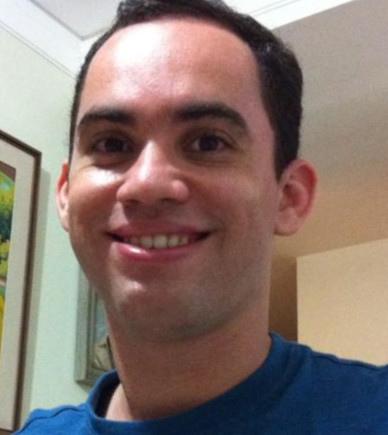
\includegraphics[scale=0.15]{imagens/prof-bruno.jpg}
		
	\end{columns}
	
	
% % 	\begin{minipage}[r]{.15\textwidth}
% % % 	\vspace{1cm}
% %     \end{minipage}
%     \hfill\begin{flushright}% or better \raggedleft see comments below
%   \vspace{-1em}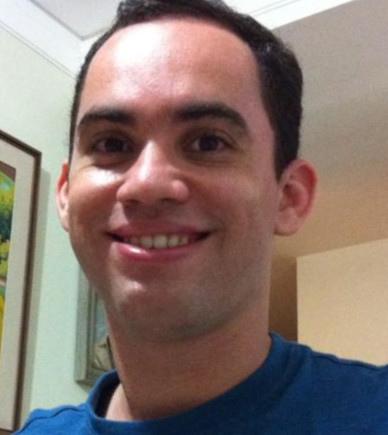
\includegraphics[scale=0.15]{imagens/prof-bruno.jpg}
%  \end{flushright}

    
%     \begin{minipage}{.85\textwidth}
%     Prof. Dr. Bruno Iran Ferreira Maciel, 37
    
%     \vspace{2mm}
%     Atualmente atuo como professor de ensino superior; Engenheiro de sistemas; e consultor de TI.
    
%     \vspace{2mm}
    
%       \fontsize{10pt}{12}\selectfont{
%     	\begin{itemize}%[<+->]  
%     	    \item Doutor em Ciência da Computação, 2015-2020
%     	    \item Mestre em Ciência da Computação, 2012-2014
%     	    \item Especialista em Engenharia e Reúso de Software, 2011-2012
%     	    \item Graduado em Sistemas de Informação, 2016-2016
%     	    \item Graduado em Ciência da Computação, 2007-2011
%     	    \item Técnico em Análise e Desenvolvimento de Software, 2007-2007
%     	    \item CV completo \url{http://bit.ly/brunomaciel-lattes}
%     	\end{itemize}
%     	}\par
%     \end{minipage}

% 	\vspace{1em}
% 	\centering
% \fontsize{20pt}{15.2}\selectfont{
% E-mail:	esuda@brunomaciel.com
% 	\vspace{1em}
% 	}\par
	
\end{frame}


\begin{frame}{}
    \fontsize{14pt}{15.2}\selectfont{
	Apresentação pessoal, integração com a turma, introdução de conceitos básicos de desenvolvimento de softwae e despertar curiosidade dos alunos sobre o tema.
	
	\vspace{1em}
	}\par
	\vspace{1em}
\end{frame}


\begin{frame}{Compromisso semanal}
%     \fontsize{14pt}{15.2}\selectfont{
% 	Datas importantes
% 	\vspace{1em}
% 	}\par
	
	\fontsize{9pt}{12}\selectfont{
	Encontros: sextas e sábados
	\begin{itemize}%[<+->]  
	    \item Período: 02/08/2024 à 30/11/2024
	    
	   % \item Laboratório: 4
	\end{itemize}
	
	\vspace{0.5em}
	Sextas
	\begin{itemize}%[<+->]  
		\item Início: 18h
		\item Térmico: 21h - Sem intervalo
		\item Térmico: 21h10 - Com intervalo de 10 minutos (a confirmar)
	\end{itemize}
	
	\vspace{0.5em}
	Sábados
	\begin{itemize}%[<+->]  

		\item Início: 9h
		\item Térmico: 12h - Sem intervalo
		\item Térmico: 12h10 - Com intervalo de 10 minutos (a confirmar)
	\end{itemize}
	
	\vspace{0.5em}
	Reposições de aulas aos Sábados no período da tarde
	\begin{itemize}%[<+->] 		
		\item Início: 14h
		\item Térmico: 17h - Sem intervalo
		\item Térmico: 17h10 - Com intervalo de 10 minutos (a confirmar)
	\end{itemize}
	
	}\par
	
	\vspace{1em}
\end{frame}


\begin{frame}{Metodologia das Aulas}
Aulas:

    \fontsize{10pt}{12}\selectfont{
    \begin{itemize}%[<+->]  
        \item 18h-19h30
        \item 19h30-21h
	\end{itemize}
	}\par
	\vspace{0.5em}
	\fontsize{12pt}{15}\selectfont{
		\begin{itemize}%[<+->]  
	    \item Resolução de dúvidas gerais e tolerância: 18h até 18h15 (15 minutos)
	    \item Revisão da aula passada: 18h15 até 18h30 (15 minutos)
	    \item Adição de novo conteúdo: 18h30 até 21h (2h30)
	   % \item Exercício em sala de aula: 21h até 21h20m (20min)
	   % \item Revisão/dúvidas do novo conteúdo: 21h20m até 21h30m (10m)
	\end{itemize}
	}\par
	\vspace{1em}
\end{frame}

%\begin{frame}{Metodologia das Avaliação}
%
%	\fontsize{12pt}{15}\selectfont{
%	\begin{itemize}%[<+->]  
%	    \item Primeira nota: (exercício + prova)
%	        \begin{itemize}%[<+->]  
%        	    \item Exercícios (peso +1)
%        	    \item Prova escrita (peso 10)
%        	\end{itemize}
%    	\item Segunda nota: (exercício + prova + seminário)
%	        \begin{itemize}%[<+->]  
%        	    \item Exercícios (peso +1)
%        	    \item Prova escrita (peso 7)
%        	    \item Seminário (peso 3)
%        	\end{itemize}
%	\end{itemize}
%	}\par
%	\vspace{1em}
%\end{frame}

%\begin{frame}{Avisos}
%
%	\fontsize{12pt}{15}\selectfont{
%	\begin{itemize}%[<+->]  
%	    \item Frequência escolar:
%	        \begin{itemize}%[<+->]  
%        	    \item Número de faltas maior que 25\% = |Reprovado por faltas|
%        	    \item Cada dia de aula faltado equivale à 4 faltas;
%        	    \item Há 15 dias de aulas no cronograma |15 = 100\%|;
%        	    \item 4 dias faltados equivale a $\pm$ 26\%.
%         	\end{itemize}
%    	\item Atraso na entrega de atividade:
%	        \begin{itemize}%[<+->]  
%        	    \item Cada dia atrasado tem penalidade de menos 10\% do peso.
%        	    \item Tempo máximo de atraso tolerado = 7 dias.
%        	\end{itemize}
%	\end{itemize}
%	}\par
%	\vspace{1em}
%\end{frame}



\begin{frame}[t]{EMENTA}
\vspace{1cm}
	\fontsize{12pt}{16}\selectfont{
	O curso tem como objetivo desenvolver as habilidades necessárias em programação, noções de padrões de desenvolvimento de software, arquitetura cliente-servidor, noções de banco de dados e frameworks back-end para que você seja capaz de projetar soluções web que sejam seguras, robustas e escaláveis, com base em tecnologias modernas e nas melhores práticas de desenvolvimento de software.
	}\par
	\vspace{1em}
\end{frame}

\begin{frame}[t]{OBJETIVO}
\vspace{1cm}
	\fontsize{12pt}{16}\selectfont{
	Compreender o funcionamento de características e arranjos básicos de desenvolvimento de software com foco em backend.
	
	
	Permitir análise crítica das questões relativas aos conceitos estudados ao longo das aulas, bem como a identificação de áreas de pesquisa voltadas para o aperfeiçoamento das técnicas e desenvolvimento de novas aplicações.
	}\par
	\vspace{1em}
\end{frame}

\begin{frame}{Competências Específicas}

	\fontsize{12pt}{15}\selectfont{
	\begin{itemize}%[<+->]
	    \item Lógica de Progamação.
	    \item Padrões de projetos.
	    \item Soft Skills.
	    \item Padrões de projetos.
	    \item POO.
	    \item Git.
	    \item Web Services.
	    \item Django.
	\end{itemize}
	}\par
	\vspace{1em}
\end{frame}


%\begin{frame}[c]{Temas para seminários}
%%Ferramentas:
%
%\vspace{2mm}
%	\fontsize{10pt}{12pt}\selectfont{
%		\begin{itemize}%[<+->]  
%			\item Apache Hadoop (HDFS) - computação distribuída voltada para clusters e processamento de grandes volumes de dados;
%			\item MapReduce - modelo para processar grandes volumes de dados em paralel;
%			\item GoogleFS ou GFS - sistema de arquivos distribuído proprietário desenvolvido pelo Google;
%			\item GFS2 - sistema de arquivos em disco compartilhado para clusters de computadores Linux;%Global File System 2
%			\item CTDB Clustered Samba;
%			\item Gluster - sistema de arquivos de rede;
%			\item técnica channel Bonding - unir redes de alta performance;
%			\item Apache Server - servidor web;
%			\item Pacemaker - gerenciado de recursos para clusters;
%			\item DRBD - Distributed Replicated Block Device - p/ dispositivos de armazenamento distribuídos;
%			\item OpenStack - Sistema Operacional da Nuvem - capaz de gerenciar os componentes de múltiplas infraestruturas virtualizadas.
%		\end{itemize}
%	}\par
%	\vspace{1em}
%\end{frame}






\begin{frame}[t]{Github das aulas}
	\vspace{7em}
	\centering
	\fontsize{16pt}{15.2}\selectfont{
	
	\url{https://github.com/brunom4ciel/material-python}
		
	}\par
	\vspace{1em}
	
	
	
\end{frame}




\begin{frame}[t]{Bibliografia básica}
    \fontsize{12pt}{15.2}\selectfont{
	\vspace{1em}
	    \begin{itemize}
	        \item \textbf{Ghetan, Giridhar. Aprendendo Padrões de Projeto em Python, 1ª Edição. Novatec. 2016.} \cite{2016:gretan}
%            \item COULOURIS, G.; DOLLIMORE, J.; KIDBERG, T. Sistemas Distribuídos Conceitos e Projetos, 4ª edição. Bookman. 2007. 
%            \item DANTAS, Mario. Computação Distribuída de Alto Desempenho: Redes, Clusters e Grids Computacionais. Axcel. 2005. 
%            \item Mais informações é possível encontrar na ementa.
	    \end{itemize}
	}\par
\end{frame}



%\begin{frame}{Google sala de aula}
%	
%    \hfill\begin{flushright}% or better \raggedleft see comments below
%	 \vspace{-10mm}\includegraphics[width=25mm]{imagens/fig-qrcode-classroom.png}
%	\end{flushright}
%
%
%%    \begin{wrapfigure}{r}{30mm}
%%    \vspace{-15mm}\qrcode[height=1in]{https://classroom.google.com}
%% 	\includegraphics[keepaspectratio=true,scale=0.4,trim=0cm 0 0 5cm]{imagens/qrcode.png}
%%	\end{wrapfigure}
%	\vspace{-15mm}
%	
%    \fontsize{14pt}{15.2}\selectfont{
%	\vspace{1em}Código da turma \fontsize{34pt}{15.2}\selectfont{fytbwcx}
%	}\par
%	\vspace{0.5em}
%
%	\fontsize{10pt}{12}\selectfont{
%	Vamos ter como recurso complementar o Google Sala de Aula [classroom]. Por lá vou deixar o material (slides, referências, atividades, etc.) que vocês vão utilizar durante o curso. Não preocupem-se, também vou deixar uma cópia do material (slides e atividades) disponível em pendrive e levarei comigo durante as aulas para os alunos que não puderem acessar o Google Classroom.
%	\vspace{1em}
%	
%	
%	
%	Como usar o google sala de aula?
%
%    Use este tutorial \url{https://www.youtube.com/watch?v=l4oSdhLS5fQ} [vídeo] para te ajudar a entender o Google Classroom.
%
%    Clique na \url{https://classroom.google.com} para entrar no Google Classroom.
%
%	}\par
%\end{frame}








	
	
	% ----------------------------------------------------------
	% ACRÔNIMO
	% ----------------------------------------------------------
	{\setbeamertemplate{footline}{} 
		\begin{frame}[allowframebreaks,noframenumbering,c]{Acrônimo}
			\vspace{2mm}
			\fontsize{11.2}{7.2}\selectfont{}
			\printglossary[type=\acronymtype,title=, toctitle=]
	\end{frame}}
	
	% ----------------------------------------------------------
	% carrega os slides das aulas
	% ----------------------------------------------------------
	\foreach\x in {\inputFilesStartValue,...,\inputFilesMaxValue}{
    \IfFileExists{aulas/0\x.tex}{\input{aulas/0\x.tex}}{\IfFileExists{aulas/00\x.tex}{\input{aulas/00\x.tex}}{}}
}

	
	
	% ----------------------------------------------------------
	% CAPA
	% ----------------------------------------------------------
	{\setbeamertemplate{footline}{} 
		\setbeamertemplate{headline}{
			\leavevmode%
			\hbox{%
				\begin{beamercolorbox}[wd=\paperwidth,ht=2.5ex,dp=1.125ex]{palette quaternary}%
				\end{beamercolorbox}%
			}
		}
		\begin{frame}[c,t]
			\maketitle
	\end{frame}}
	
	
	
	% ----------------------------------------------------------
	% GLOSSÁRIO
	% ----------------------------------------------------------
	\begin{frame}[c,allowframebreaks,noframenumbering]{Exercícios}
		\justify
		\printglossary[title=, toctitle=]
	\end{frame}
	
	
	
	% ----------------------------------------------------------
	% REFERÊNCIAS
	% ----------------------------------------------------------
	\part{Referências}
	\frame{\partpage}
	\nocite{*}
	{
		\setbeamertemplate{footline}{} 
		\setbeamertemplate{headline}{
			\leavevmode%
			\hbox{%
				\begin{beamercolorbox}[wd=\paperwidth,ht=4.5ex,dp=1.125ex]{palette quaternary}%
				\end{beamercolorbox}%
			}
		}
		\begin{frame}[allowframebreaks,noframenumbering]{Referências}
			\fontsize{11.2}{7.2}\selectfont{}
			\bibliographystyle{abbrvnat} %\usepackage{natbib}
			\bibliography{referencias}
			% \printbibliography
		\end{frame}
	}
	
	
	
	
	
	% ----------------------------------------------------------
	% incluir ementa dentro do material
	% ----------------------------------------------------------
	% \setbeamertemplate{background canvas}{}
	% \include{plano-aulas}
	% \includepdf[pages=-,fitpaper]{outros/ementa.pdf}
	% % noautoscale
	% % fitpaper
	% %
	% %
	% %*******************************************************
	
	
	
\end{document}
